\RequirePackage{plautopatch}
\documentclass[a4paper,papersize,uplatex,dvipdfmx,10pt]{jsarticle}
%\documentclass[a4paper,papersize,uplatex,dvipdfmx,10pt,twocollumn]{jsarticle} % 二段組にするならこちら

%package類
%%%%%%%%%%%%%%%%%%%%
\usepackage[utf8]{inputenc}
\usepackage[T1]{fontenc}
\usepackage[prefernoncjk]{pxcjkcat}
\usepackage[scaled=1.05,helvratio=0.95]{newtxtext}
\usepackage[dvipdfmx]{color}

\usepackage[colorlinks=true,allcolors=blue]{hyperref}
%\usepackage[dvipdfmx,hidelinks]{hyperref} % 紙に印刷するときは青文字リンクは消す。

\usepackage{pxjahyper} % 文字化け防止
\usepackage{array,amsmath,amssymb,bm,cases} % 数式でよく使うもの
\usepackage[dvipdfmx]{graphicx} % 画像使用
\usepackage{url} % \url{} の間にurlを挟む

%\usepackage{natbib}
\usepackage[numbers]{natbib} % bibliographystyleを「jplain」にした時、エラーが出るならこちらを試す

\usepackage{ascmac} % itembox環境やscreen環境などの枠関係の環境

\usepackage{enumerate} % enumerate環境

\usepackage[nottoc,notlot,notlof]{tocbibind} % bibliography を目次に追加

%\usepackage{mathtools} % dcases環境 % 普段あまり使わないからコメントアウト

\usepackage[nooneline]{subfigure}
\subfiguretopcaptrue % subfigure環境で使う

%\usepackage{comment}
% ソースの中に説明書きするときに使う
% この環境下のものはコンパイルされない

\allowdisplaybreaks[4] % 数式がページをまたぐのを許す

\usepackage{listings,jvlisting} %日本語のコメントアウトをする場合jvlisting(もしくはjlisting)が必要
%ここからソースコードの表示に関する設定
\lstset{
  basicstyle={\ttfamily},
  identifierstyle={\small},
  commentstyle={\smallitshape},
  keywordstyle={\small\bfseries},
  ndkeywordstyle={\small},
  stringstyle={\small\ttfamily},
  frame={tb},
  breaklines=true,
  columns=[l]{fullflexible},
  numbers=left,
  xrightmargin=0zw,
  xleftmargin=3zw,
  numberstyle={\scriptsize},
  stepnumber=1,
  numbersep=1zw,
  lineskip=-0.5ex
}
%ここまでソースコードの表示に関する設定
% https://qiita.com/ta_b0_/items/2619d5927492edbb5b03
% を使わせて頂いています。

%newcommand類
%%%%%%%%%%%%%%%%%%%%
\newcommand{\bs}{\symbol{92}} %backslash
\newcommand{\red}[1]{\textcolor{red}{#1}} %文字色赤
\newcommand{\blue}[1]{\textcolor{blue}{#1}} %文字色青
\newcommand{\green}[1]{\textcolor{green}{#1}} %文字色緑
\newcommand{\ured}[1]{\textcolor{red}{\underline{\textcolor{black}{#1}}}} %下線赤
\newcommand{\ugreen}[1]{\textcolor{green}{\underline{\textcolor{black}{#1}}}} %下線緑
\newcommand{\ublue}[1]{\textcolor{blue}{\underline{\textcolor{black}{#1}}}} %下線青
%%%%%%%%%%%%%%%%%%%%

\title{タイトル名}
%\title{\vspace{-3cm}タイトル名} % タイトル上のスペースを減らしたい場合はこっち

\author{東北大学宇宙地球物理学科天文学コース\\B9SB0000\,\,天文太郎}
\date{\today}

\begin{document}
\maketitle

\nocite{*}
% 文書内で引用していないものを、参考文献に載せる場合に\nocite{}を使う。
% 例えば、cite keyを「hogehoge」にしている文献を引用していなくても参考文献に載せるなら
% \nocite{hogehoge}
% とする。
% ここではワイルドカード「*」を使っているので、.bibに載せている文献は何もかも参考文献として表示させる。

\section{はじめに} %
\LaTeX を使う人が増えそうなので、簡単に説明を付属させたテンプレートを作りました。これをたたき台にして、適当に弄りこんにゃくして下さい。\par
一応、参考になるように\texttt{main.tex}内には、コメントアウトなどで説明を踏まえつつ色々とコマンドを使っているので、\texttt{main.pdf}と一緒に見比べてコマンドの効果を確認しながら、使えそうだなってのは使ってください。コード全体に関して僕自身が著作権を主張するようなものは存在しないので、特別に表記しているもの以外については、勝手に使って大丈夫だと思います。\par
何かしら不具合があればGitHubにissue\footnote{\url{https://github.com/NaokiMatsumoto0209/templete_astr_jsarticle/issues}}を立ててもらえれば助かります。issues機能を使った経験がないので、その練習にしたいです。

\section{文章について} %
文章の書き方という言葉には2種類ほどあると思いますが、「わかりやすい文章の書き方」は僕も勉強中なので、別な本とかを参照して下さい\footnote{文章が\textbf{書けない}という人はそもそも\LaTeX を使わないでしょう。}。\par
ちなみに、コード中に先ほどから出現している\texttt{\bs par}は改段落するコマンドです。1行空けて書くことでも改段落できますが、コードが長くなるので\footnote{気のせい}僕は使わなくなりました。\par

\subsection{数式表現} %%
\LaTeX を使う1番の目的は数式を書くためだと思います。数式を書くときには数式環境を使うはずです。いくつか簡単に説明します。

\subsubsection{文中の数式} %%%
文中で数式を使う場合は\texttt{\$}を使います。実際に見せた方が早いので、実際に使ってみます。

\begin{screen}
  無偏光の場合のThomson散乱について考える。無偏光波は2つの互いに独立な直線偏光波の重ね合わせとみなせる。ここで、$\bm{\epsilon}_{1}$を入射方向と散乱方向$\bm{n}$を含む平面内にとり、$\bm{\epsilon}_{2}$をこの平面に垂直にとる。$\Theta$を$\bm{\epsilon}_{1}$と$\bm{n}$の間の角、$\theta = \Theta - \pi/2$とする。すると、$\theta$は入射波と散乱波の間の角となる。
\end{screen}

例えば、上の文中では$\theta = \Theta - \pi/2$は\texttt{\$ \bs theta = \bs Theta - \bs pi/2 \$}と書いています。このように\texttt{\$...\$}で数式表現を挟むことで、文中で数式を使うことができます。\par
ちなみに、分数を\texttt{\bs frac}を使わずに書いている理由は、$\frac{1}{2}$という形がダサいように感じられるからです。$1/2$と書いた方が良いように思います。まあここら辺は人の好みかもしれないですけど。

\subsubsection{文外の数式} %%%
文外で数式を使う場合は僕は一貫して\texttt{align}環境しか使っていないですが、\texttt{equation}環境や\texttt{\$\$...\$\$}で挟む方法などもあります。僕が\texttt{align}環境しか使わないのは、改行もできるし、改行しなくてもいいし、数式番号も楽に消せるしで、他をわざわざ選ぶ理由が無いように感じられるからです。実際に使ってみます。

\begin{screen}
  無偏光の場合の微分散乱断面積は2つの直線偏光波の微分散乱断面積の平均と捉えることができる。
  \begin{align}
    \left( \frac{\mathrm{d}\sigma}{\mathrm{d}\Omega} \right)_{\mathrm{unpolarized}} &=
    \frac{1}{2}\left[ \left( \frac{\mathrm{d}\sigma(\Theta)}{\mathrm{d}\Omega} \right)_{\mathrm{polarized}} + \left( \frac{\mathrm{d}\sigma(\pi / 2)}{\mathrm{d}\Omega} \right)_{\mathrm{polarized}} \right]\notag\\
    &= \frac{1}{2}r_{0}^{2}\left( 1+\sin^{2}\Theta \right)\notag\\
    &= \frac{1}{2}r_{0}^{2}\left( 1+\cos^{2}\theta \right)
  \end{align}
  これが無偏光波が入射方向に対して角度$\theta$の方向に散乱される場合の微分散乱断面積で、\textbf{トムソンの公式}と呼ばれる。
  \begin{itembox}[l]{Thomson formula}
    \begin{align*}
      \left( \frac{\mathrm{d}\sigma}{\mathrm{d}\Omega} \right)_{\mathrm{unpolarized}} = \frac{1}{2}r_{0}^{2}\left( 1+\cos^{2}\theta \right)
    \end{align*}
  \end{itembox}
  \begin{itemize}
    \item トムソンの公式は$\theta$に対して対称であるから、前方に散乱される場合と後方に散乱される場合で対称となる。
    \item 散乱断面積$\sigma_{\mathrm{T}}$は直線偏光の場合と同様に全立体角積分すればよい:
    \begin{align}
      \sigma_{\mathrm{T}} &= \frac{1}{2}r_{0}^{2} \int^{2\pi}_{0}\mathrm{d}\phi \int^{\pi}_{0}\mathrm{d}\theta\, \left( 1+\cos^{2}\theta \right) \sin\theta\notag\\
      &= \frac{8}{3}\pi r_{0}^{2}\label{eq:sanran_unpol}
    \end{align}
  \end{itemize}
\end{screen}

\subsection{画像} %%
ここからは、画像や表、コードの挿入の方法について説明します。一応、いつも利用しているテンプレートは同梱の\texttt{fig\_tab\_temp.tex}にあるので、使って下さい。\par
画像の挿入方法ですが、\texttt{figure}環境を使います。実際に画像を挿入してみると図~\ref{fig:co_vs_ci}となります。
\begin{figure}
  \centering % centering環境は、ページの中央に対象を置くようにする命令です。
  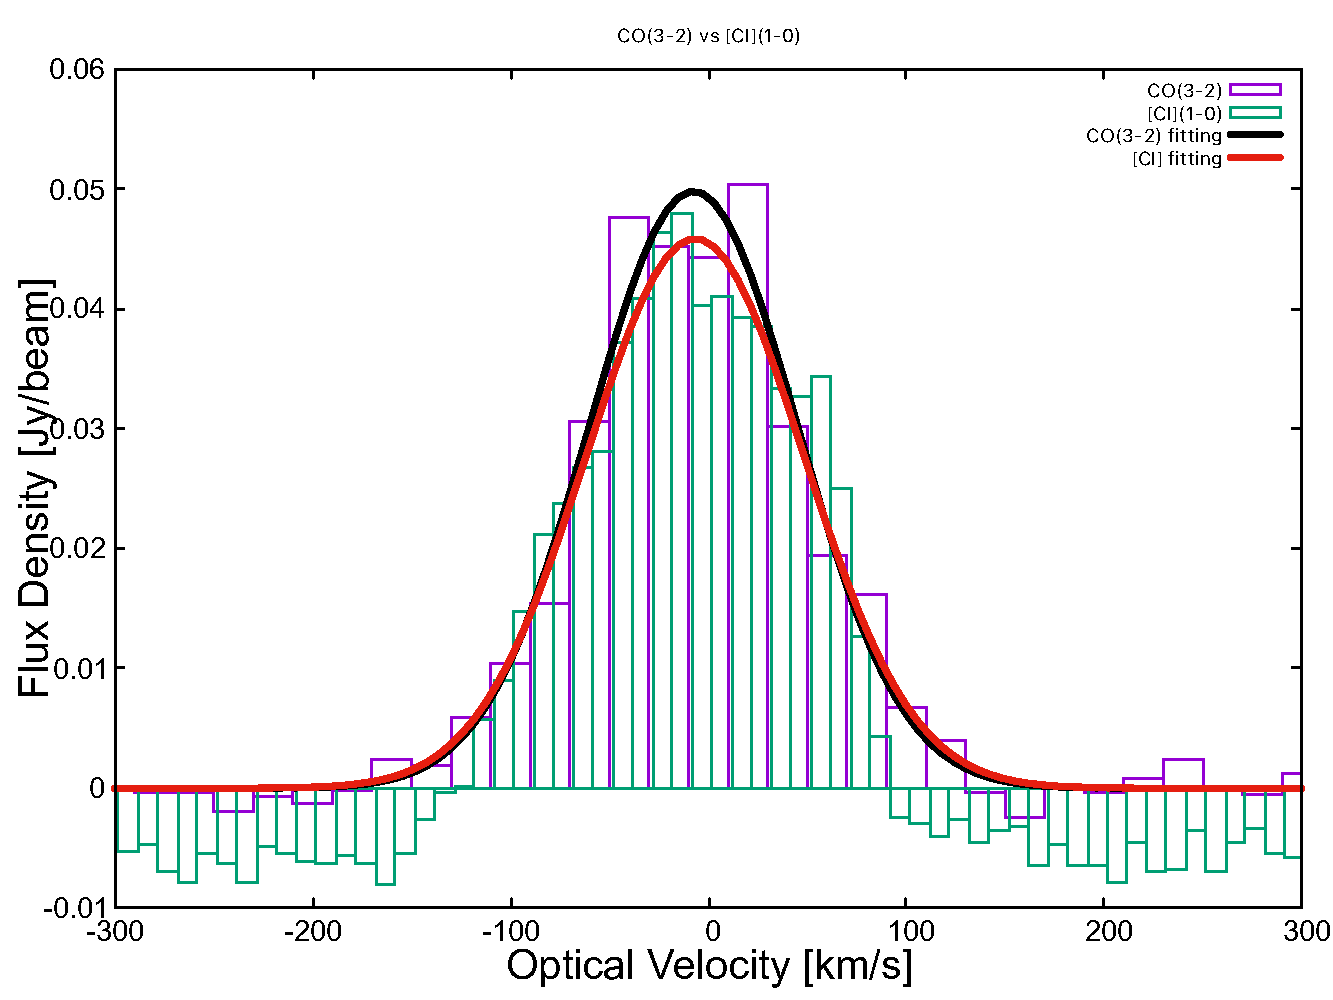
\includegraphics[width=0.5\linewidth]{./fig/test.pdf}
  %[]で囲んだ部分は画像の大きさを指定します。
  \caption[Circinus銀河の中心部での輝線強度比]{Circinus銀河の$\mathrm{CO}(3-2)$と$[\mathrm{C}\mathrm{I}]$の中心部での輝線強度比}
  %[]のオプションは画像リストを利用する際のキャプションになるもので、画像自体のキャプションにはなりません。
  %jsarticleでは画像リストを使わなければならないような大規模な文章にはなりにくいと思いますが、個人的なお作法として入れているだけです。
  %ちなみに、画像リストは「\listoffigures」を「\maketitle」の下あたりに書くだけです。
  \label{fig:co_vs_ci}
\end{figure}
コードとしては
\begin{verbatim}
  \begin{figure}
    \centering
    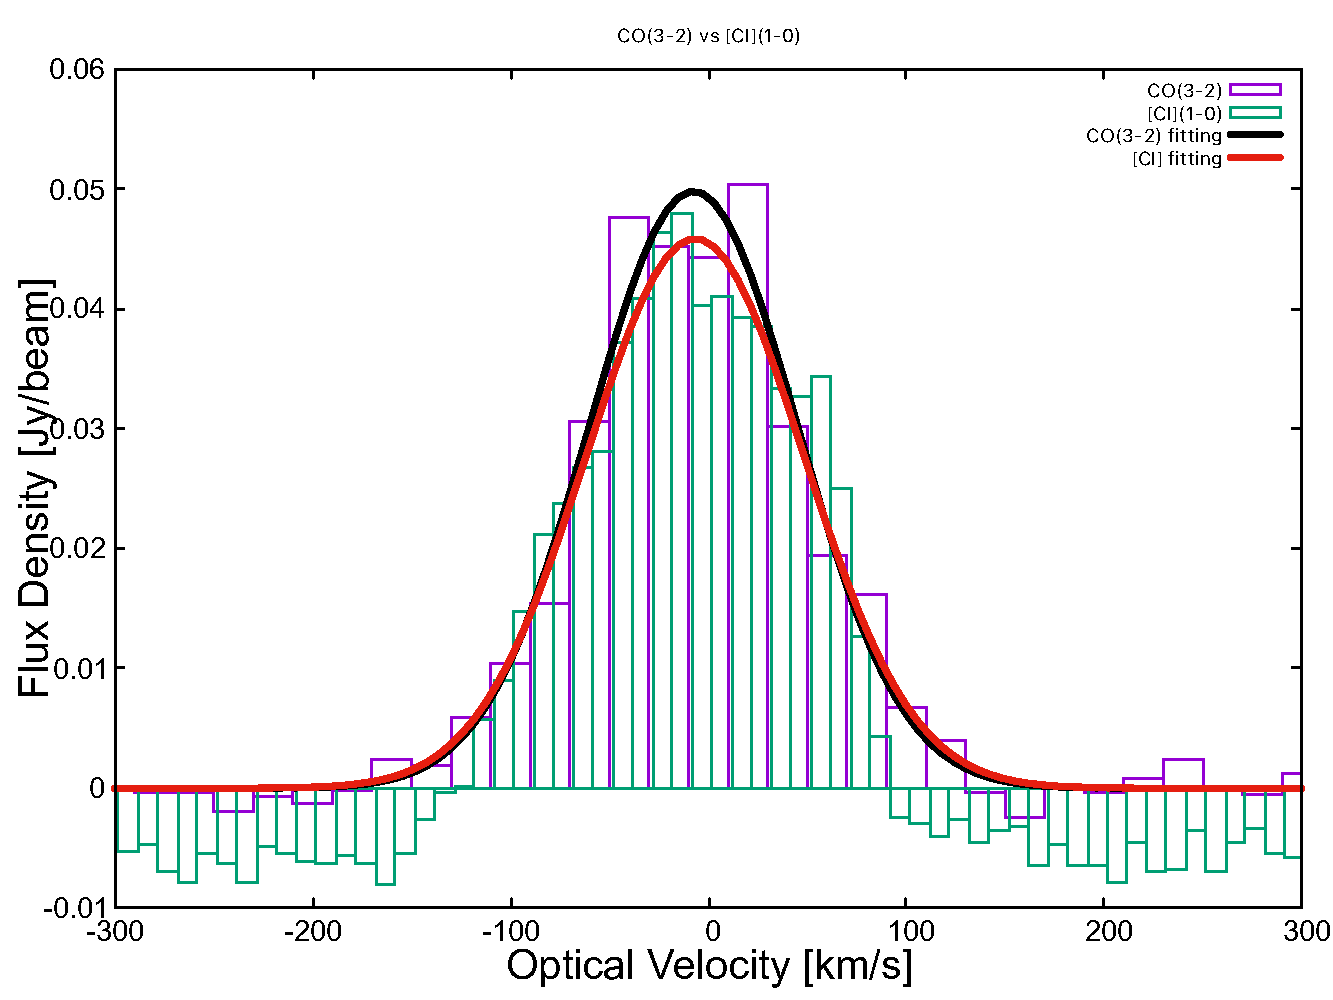
\includegraphics[width=0.5\linewidth]{fig/test.pdf}
    \caption[Circinus銀河の中心部での輝線強度比]{Circinus銀河の$\mathrm{CO}(3-2)$と$[\mathrm{C}\mathrm{I}]$の中心部での輝線強度比}
    \label{fig:co_vs_ci}
  \end{figure}
\end{verbatim}
となっています。挿入される位置はデフォルトではページの上部になるはずです。ここが今までWordを使ってきた方にとって混乱するポイントの1つだと個人的に思っていて、\LaTeX{}ではあまり画像位置の指定をしません\footnote{私個人の大変短い経験によるものであり、例えば論文などのフォーマットでそのような指定がなされる可能性があります。その場合は適宜、状況にあった画像挿入の方法、位置指定の方法を調べてください。}。どうしても"ここ"に挿入したいという場合は、\texttt{\bs begin\{figure\}[h]}と指定します。\texttt{h}は「here」の意味です。\texttt{b}はページの下になったりと、4種類くらい指定方法があり優先順位があります。しかし、滅多に使ってないのでここでは詳細に説明しません。今回は\texttt{test.pdf}を挿入しましたが、その他の画像形式も挿入することができます。ここでは\texttt{subfigure}環境を使用してそれぞれの画像形式を並べてみます。左から\texttt{.pdf}、\texttt{.png}、\texttt{.jpg}です。
\begin{figure}
  \centering
  \subfigure[]{%
  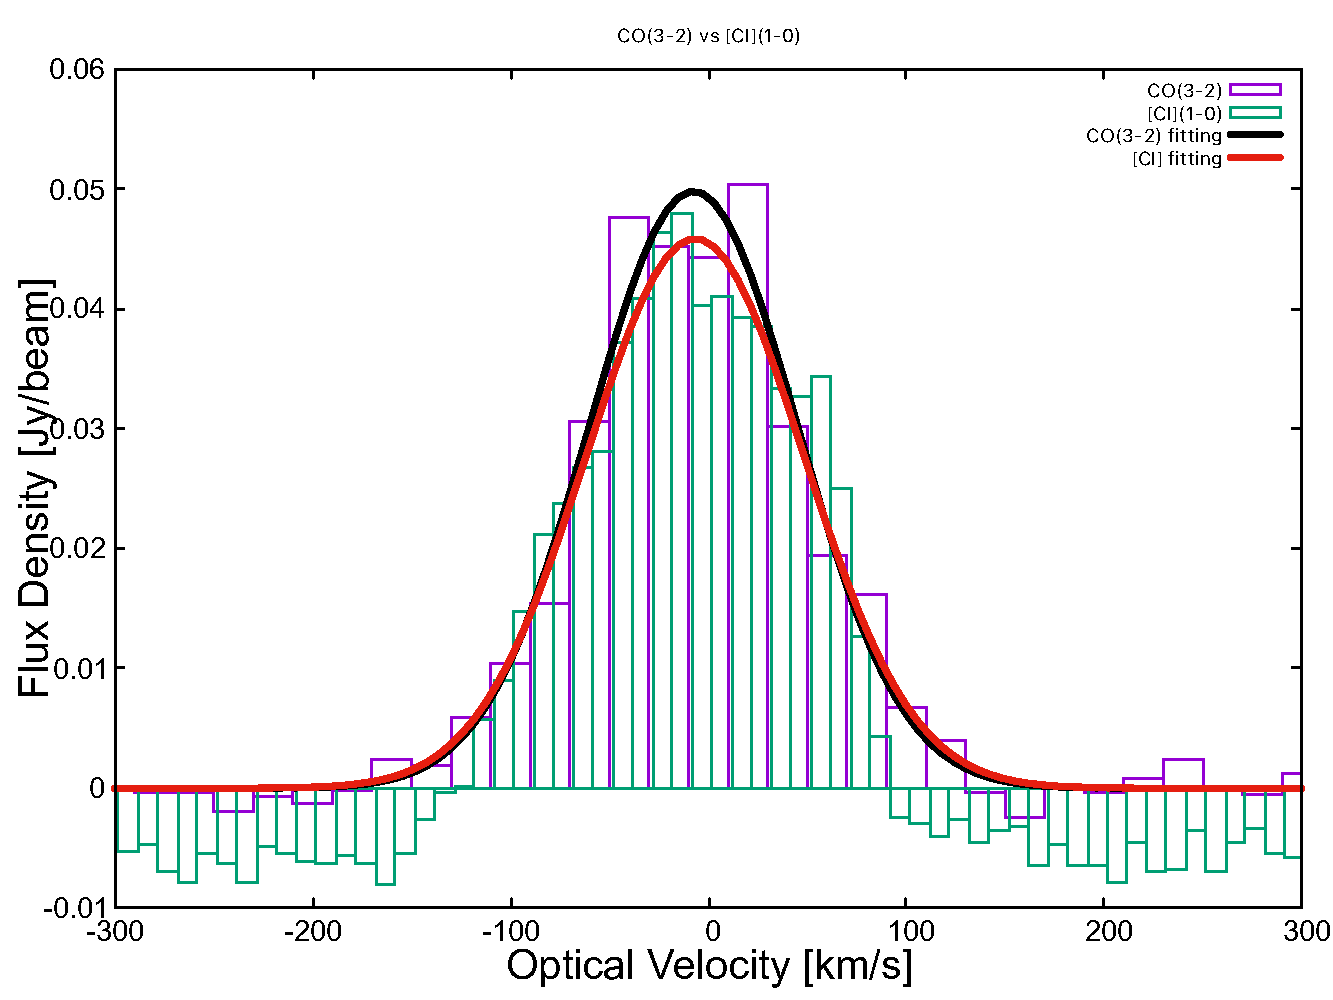
\includegraphics[width=.3\textwidth,clip]{./fig/test.pdf}%
  \label{fig:co_vs_ci_pdf}%
  }%
  \subfigure[]{%
  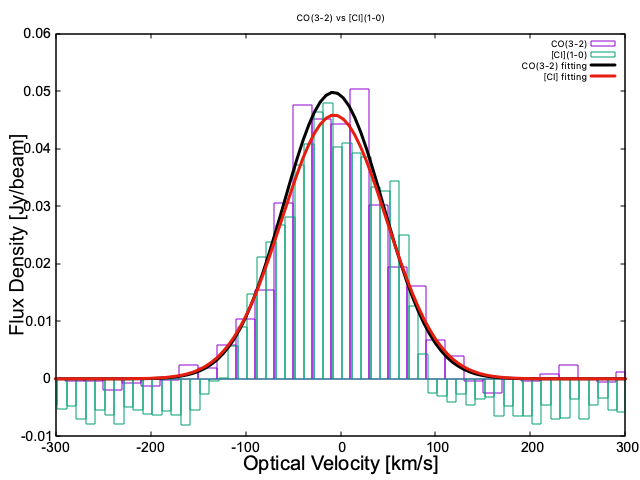
\includegraphics[width=.3\textwidth,clip]{./fig/test.png}%
  \label{fig:co_vs_ci_png}%
  }%
  \subfigure[]{%
  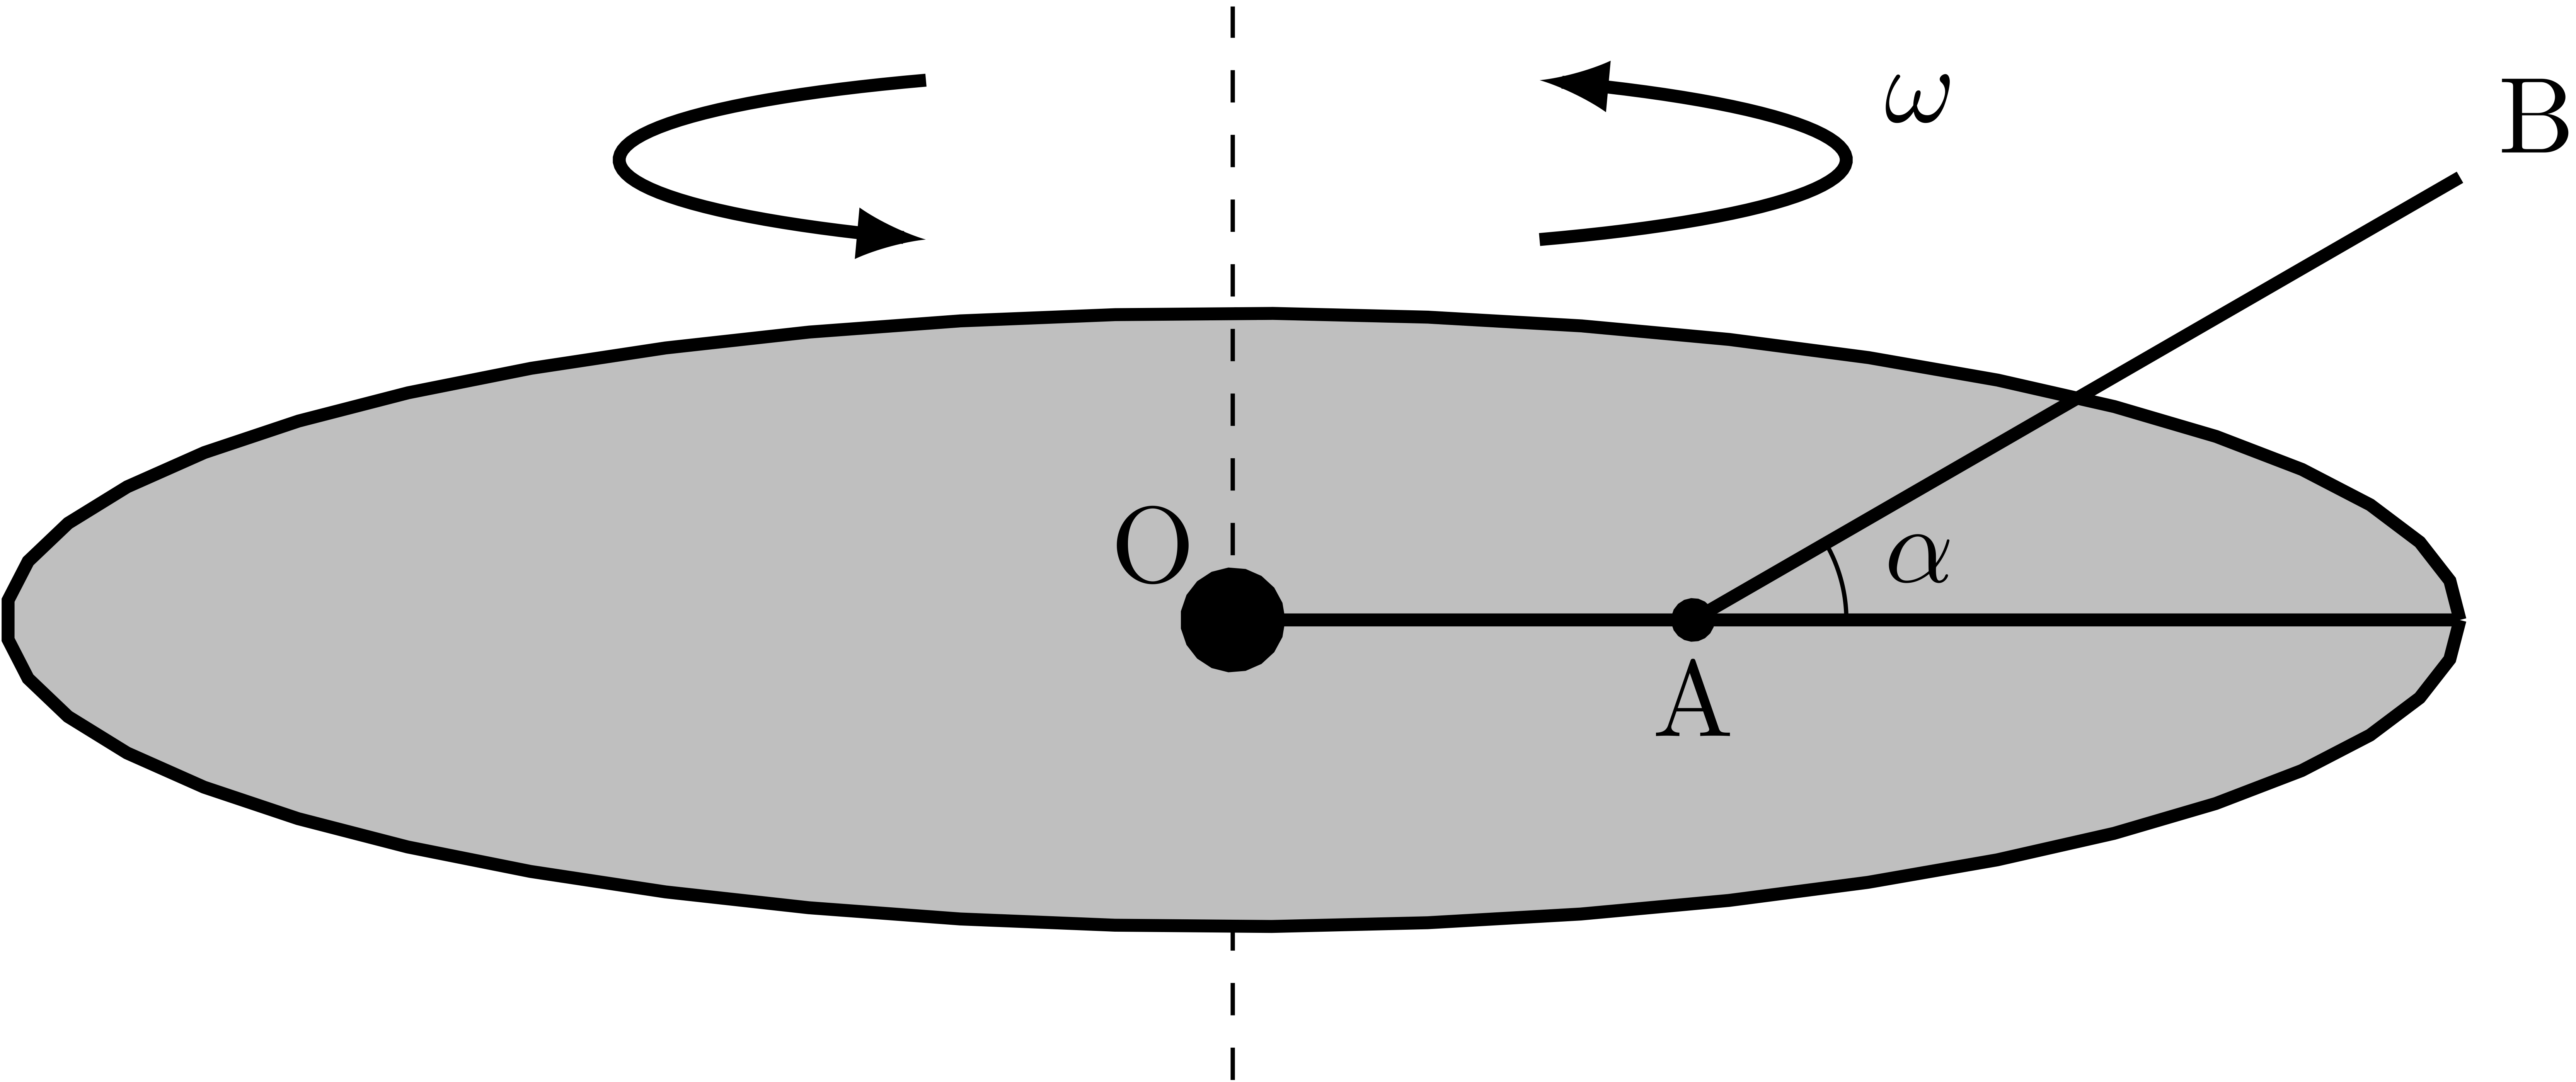
\includegraphics[width=.3\textwidth,clip]{./fig/test.jpg}%
  \label{fig:co_vs_ci_jpg}%
  }
  \caption[\texttt{subfigure}環境による画像挿入]{\texttt{subfigure}環境による画像挿入。(a)pdf形式、(b)png形式、(c)jpg形式}
  \label{fig:co_vs_ci_sb}
\end{figure}
別に意地悪して解像度を落としている訳ではないのですが、\texttt{.pdf}が解像度が良いのに比べて他2つは解像度が悪くなっています。\texttt{png}や\texttt{jpg}の仕組み上仕方ないことなのですが、\texttt{pdf}の方がファイルも軽いですし、特段の事情がない限りは\texttt{pdf}を使った方が良いと思います。

\subsection{表} %%

\subsection{コード} %%

\subsection{参考文献の表示の仕方}
参考文献を表示するために、\BibTeX を使っています。\par
活動銀河核は面白い!!!!\cite{1130000796831041920}として引用したりします。日本人の名前が「天文太郎」ではなく「太郎天文」の順になってしまっています。この場合、\texttt{\bs bibliographystyle\{jplain\}}の\texttt{\{ \}}の内部を\texttt{\{jecon\}}に変更し、\texttt{\bs usepackage[numbers]\{natbib\}}から\texttt{[numbers]}のオプションを消します。これは、ShiroTakedaさんが作られた\texttt{jecon.bst}という引用スタイルを利用するものです\footnote{\url{https://github.com/ShiroTakeda/jecon-bst}}。すると、
\begin{screen}
  活動銀河核は面白い!!!!\blue{Peterson 他}(\blue{2010})
\end{screen}
となります。どちらが良いかは好みで決めて下さい。

\section{終わりに} %

\renewcommand{\bibname}{参考文献}
%\bibliographystyle{jecon}
\bibliographystyle{jplain}
\bibliography{thesis}
\end{document}
